\documentclass{article}
\usepackage[utf8]{inputenc}
\usepackage{graphicx}
\usepackage{float}
\usepackage[justification=centering]{caption}
\usepackage{subcaption}
\graphicspath{ {./images/}}
\usepackage{listings}


\title{Report for final project, MNXB01}
\author{by Philip Siemund}
\date{2019-11-06}

\begin{document}

\maketitle

The goal of the project was to analyze data from the Swedish Meteorological and Hydrological Institute (SMHI). The data consisted of air temperature measurements from different towns in Sweden. The file format of the files containing the data was CSV. Figure 1 shows a screenshot of the file associated with Lund. 

\begin{figure}[h]
\centering
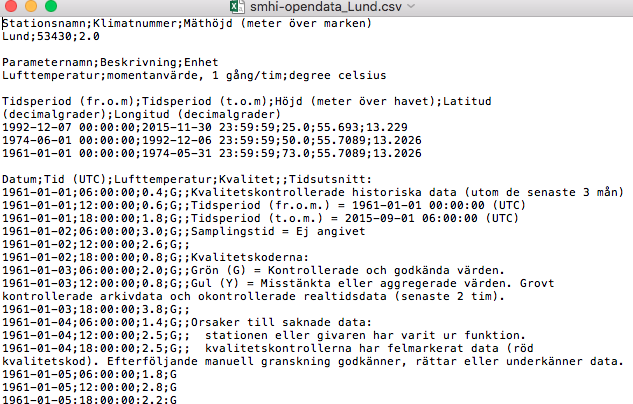
\includegraphics[scale=0.4]{Lund0}
\caption{The raw data stored in a CSV file.}
\end{figure}

To extract only the measurements of the file, that is, all that follows after the line starting with "Datum; ..." and only the first four columns (using the field separator ";" for the definition of a column), a bash script tempdata.sh was written and executed. This script would extract the relevant data and save it to a new file data\_for\_town.txt. The script went through a couple of drafts, yielding different outputs as shown in figure 2.

\begin{figure}[H]
\centering
\begin{subfigure}[h]{1\textwidth}
\centering
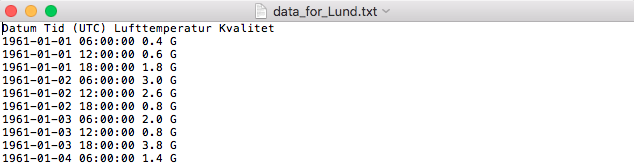
\includegraphics[width=\textwidth]{Lund1} 
\caption{} \label{figa}
\end{subfigure}

\begin{subfigure}[h]{1\textwidth}
\centering
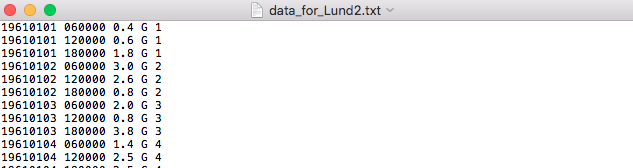
\includegraphics[width=\textwidth]{Lund2} 
\caption{} \label{figb}
\end{subfigure}


\begin{subfigure}[h]{1\textwidth}
\centering
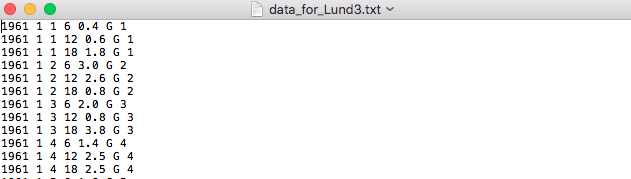
\includegraphics[width=\textwidth]{Lund3} 
\caption{} \label{figc}
\end{subfigure}

\caption{Different outputs of tempdata.sh; from earlier drafts, \ref{figa} and \ref{figb}, and final draft, \ref{figc}.}
\end{figure}
The last column in \ref{figb} and \ref{figc} specifies the day number of the year, i.e. a number between 1 and 365/366. This was achieved by creating a UNIX timestamp in tempdata.sh, which, by the way, used the single command GNU awk to format the data (see figure 3). 

\begin{figure}[H]
\centering
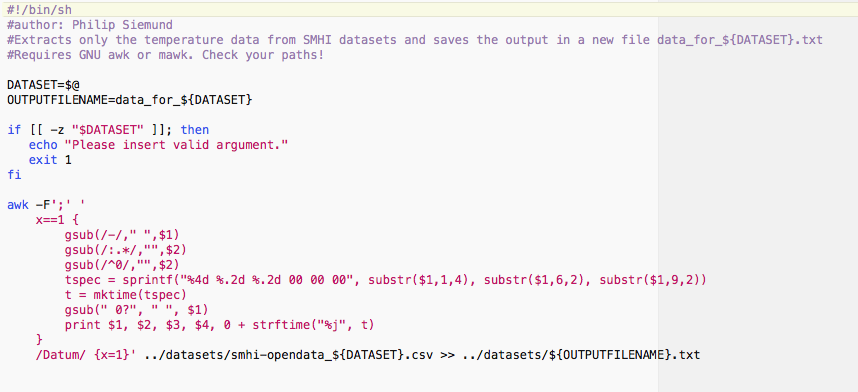
\includegraphics[scale=0.4]{Codetemp.png}
\caption{tempdata.sh.}
\end{figure}

The purpose behind tempdata.sh was to make the data more accessible. Incuding the header fstream in a given C file, one could simply stream the different datatypes in the file data\_for\_town.txt onto corresponding variables in a while-loop. The data of interest could be specified by including conditional statements in the while-loop.

The file analyze\_data.C exemplifies this (see figure 4). If one compiles the file in the data analysis tool ROOT and calls the function temPerDay(), it produces a histogram showing the temperature per day in a town at a given hour a given year. Some such histograms are shown in figure 5. 
\begin{figure}[H]
\centering
\begin{subfigure}[h]{1\textwidth}
\centering
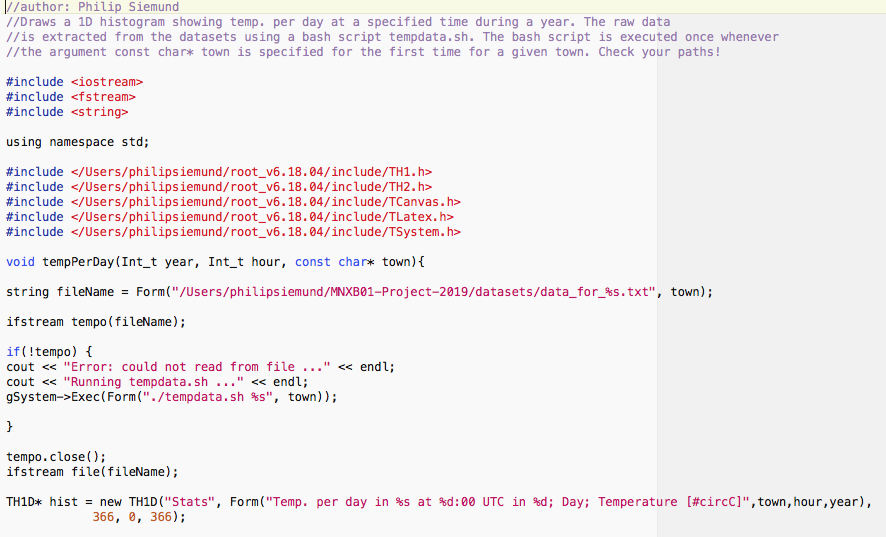
\includegraphics[width=\textwidth]{CodeAn1.png} 
\caption{} \label{figA}
\end{subfigure}

\begin{subfigure}[h]{1\textwidth}
\centering
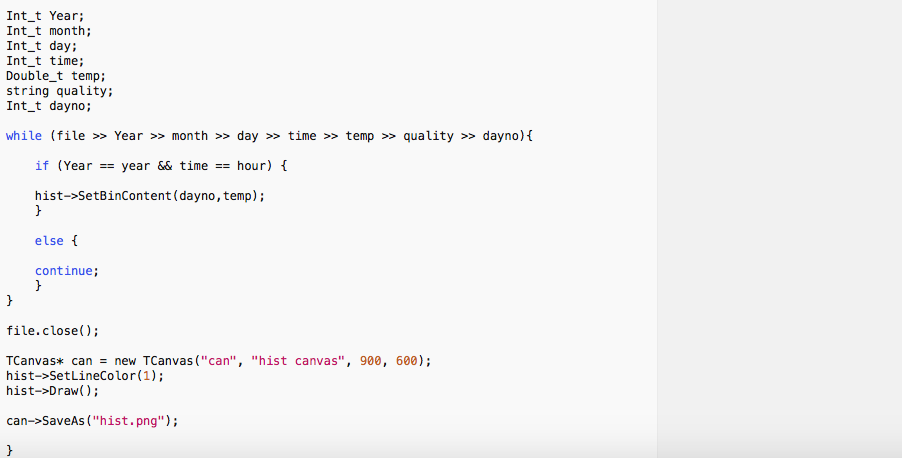
\includegraphics[width=\textwidth]{CodeAn2.png} 
\caption{} \label{figB}
\end{subfigure}
\caption{analyze\_data.C.}
\end{figure}

\begin{figure}[H]
\centering
\begin{subfigure}[h]{0.8\textwidth}
\centering
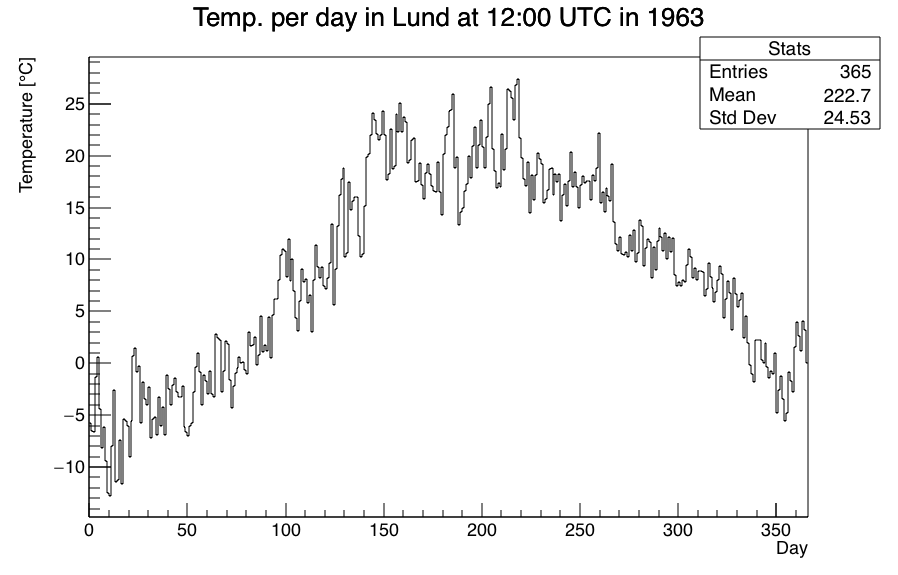
\includegraphics[width=\textwidth]{Lund12UTC1963.png} 
\caption{} \label{figAA}
\end{subfigure}

\begin{subfigure}[h]{0.8\textwidth}
\centering
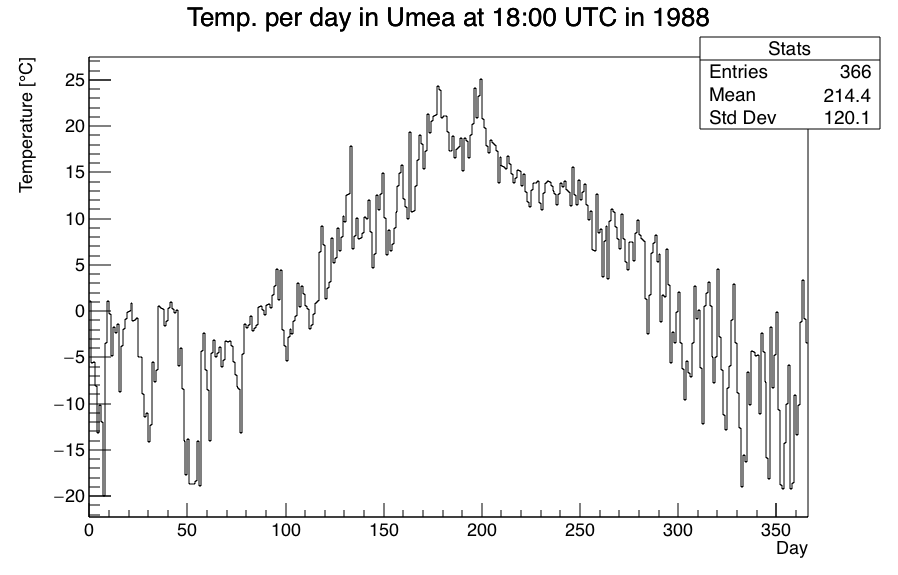
\includegraphics[width=\textwidth]{Umea18UTC1988.png} 
\caption{} \label{figBB}
\end{subfigure}

\begin{subfigure}[h]{0.8\textwidth}
\centering
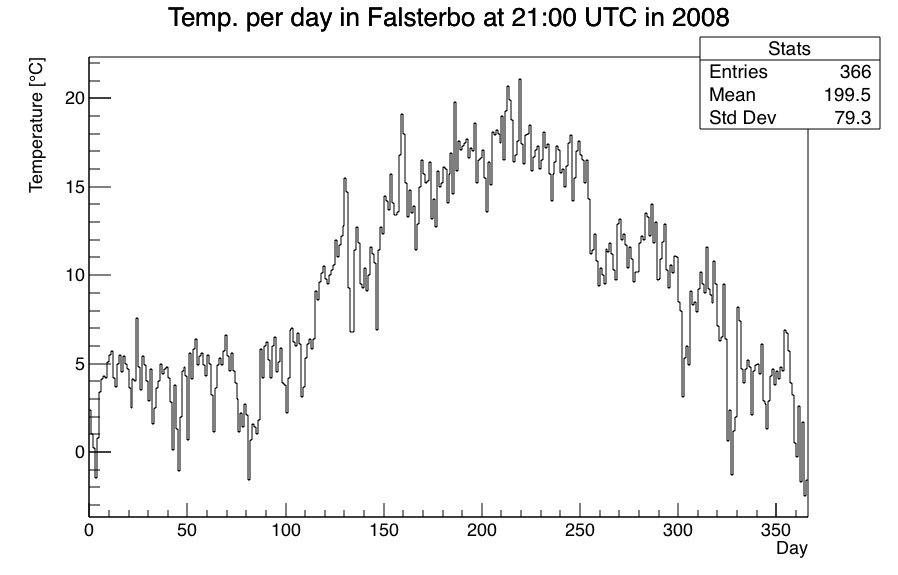
\includegraphics[width=\textwidth]{Falsterbo21UTC2008.png} 
\caption{} \label{figCC}
\end{subfigure}

\caption{Example output of analyze\_data.C.}
\end{figure}

\end{document}
